    
  \begin{frame}{Inspiracija}
  	\vspace{3em}
  	\twocolumns {
  		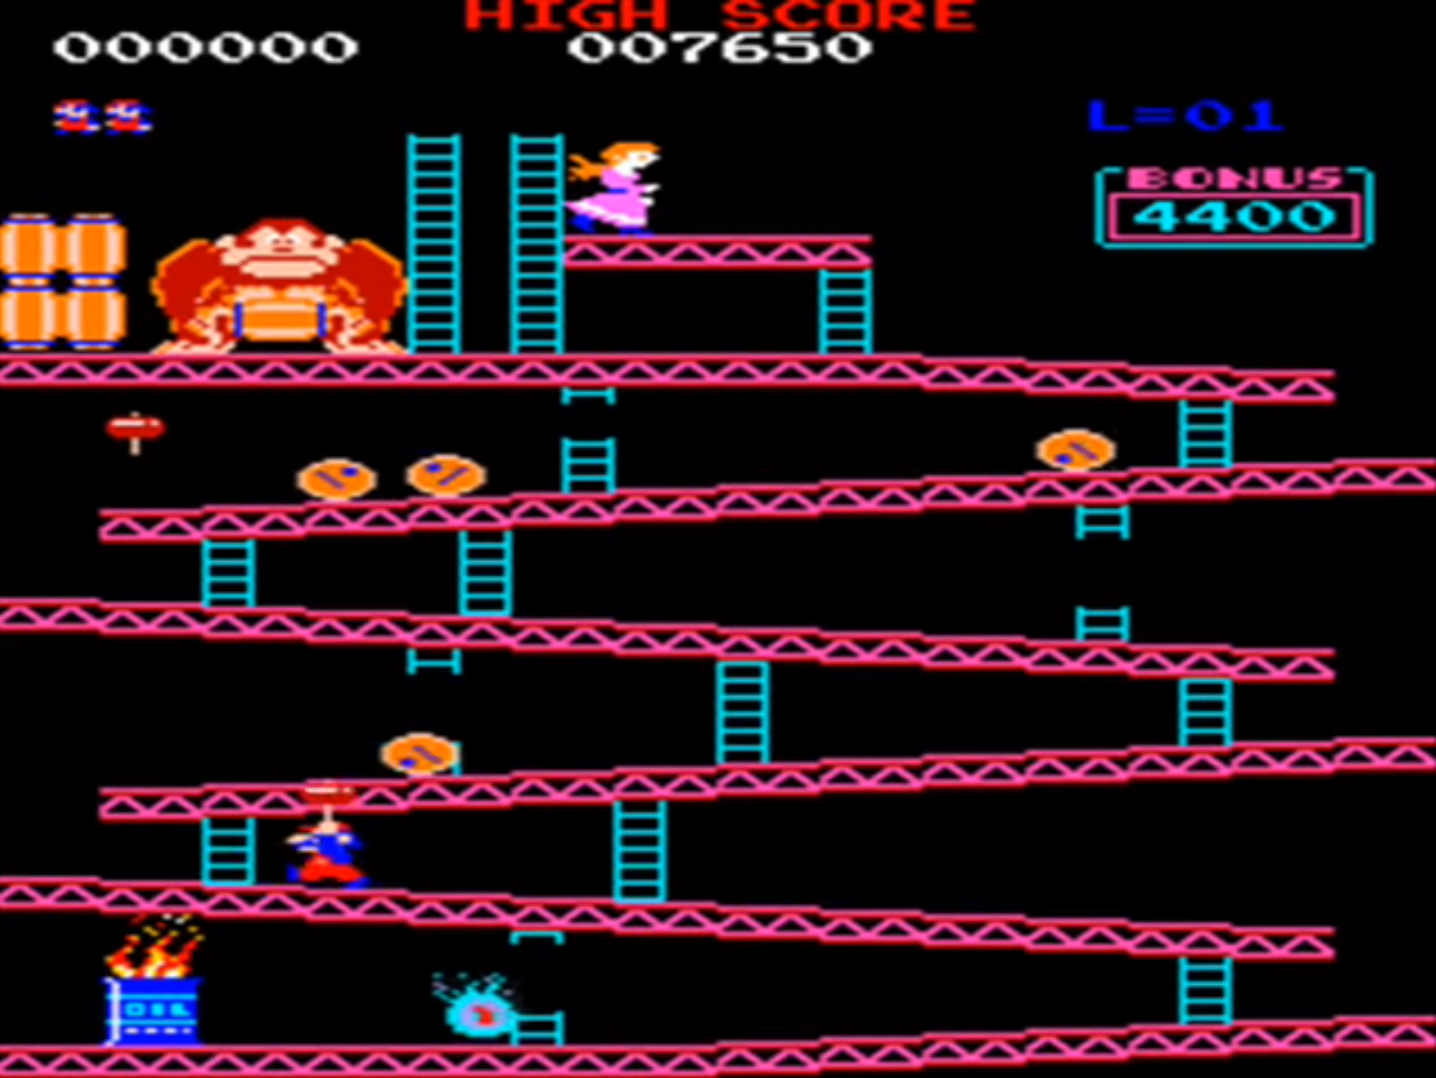
\includegraphics[width=1.2\textwidth]{slike/donkeykong_game}
  	} {
  	  \vspace{1em}
	  \hspace{3em}\fbox{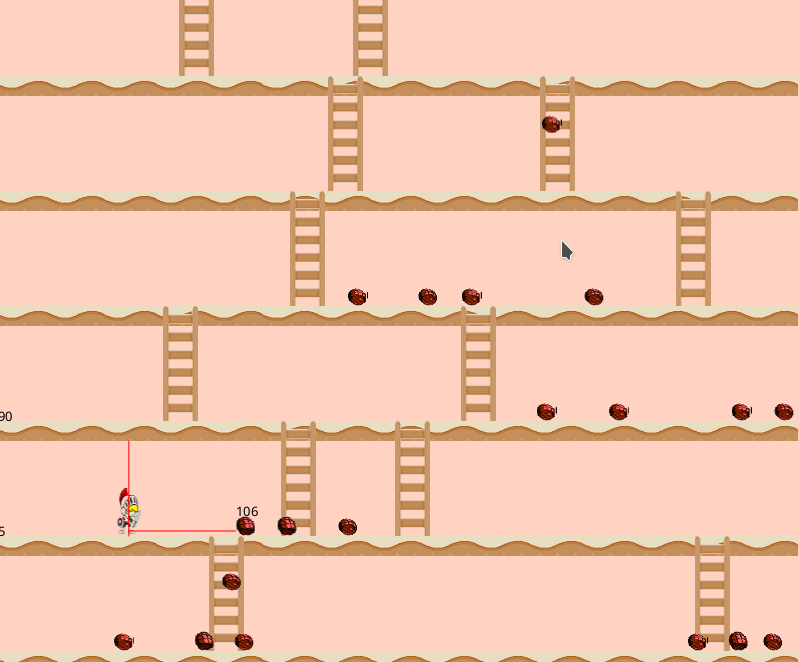
\includegraphics[width=0.7\textwidth]{slike/donquixote_game}}
  	}
  \end{frame}

	\begin{frame}{Inspiracija}
		\hspace{4em}\fbox{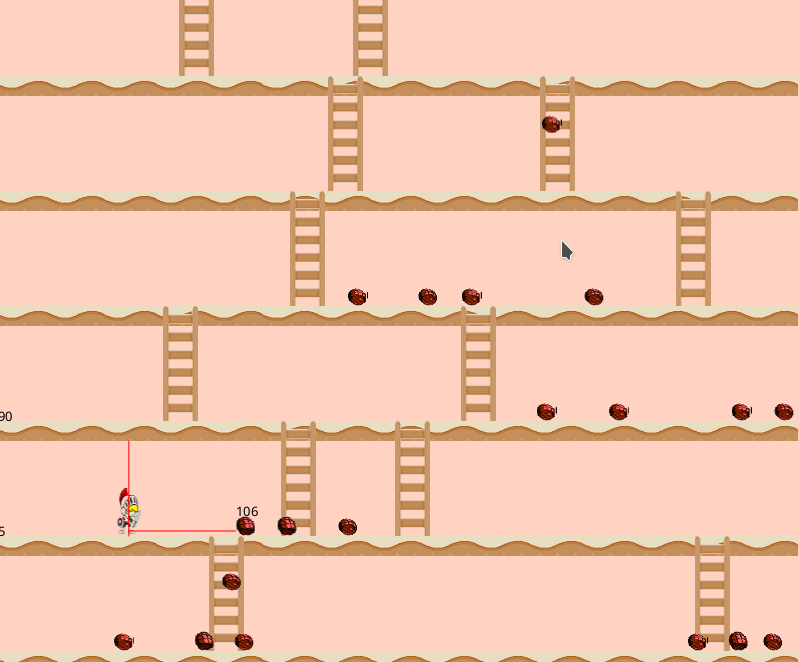
\includegraphics[width=0.7\textwidth]{slike/donquixote_game}}
	\end{frame}

  \begin{frame}{Pokretački sklop (eng. \textit{Game engine})}
  	\begin{itemize}
  		\item Diskretni otkucaji sata (eng. \textit{ticks})
  		\item Stroj stanja (eng. \textit{State machine}), oblikovni obrazac promatrač
  		\item 4 koraka:
  		\begin{enumerate}
  			\item Izračun pomaka igrača i svih ostalih objekata
  			\item Korekcija pomaka
  			\item Izračun kolizija svih objekata međusobno (uključujući i igrača)
  			\item Izračun novih brzina svih objekata 
  		\end{enumerate}
  	\end{itemize}
  	\hspace{5em}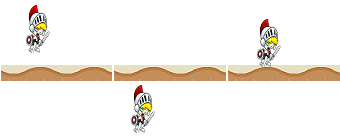
\includegraphics[width=0.65\textwidth]{slike/positionCorrection}
  \end{frame}

  \begin{frame}{Pravila igre i potezi}
  \end{frame}

  \begin{frame}{Ulazni podaci umjetnom igraču na temelju sudara zraka}
  \end{frame}
